% --- Documentclass specifications ---
\documentclass[italian]{tktltiki2}
\linespread{1.3}

% --- General packages ---
\usepackage[utf8]{inputenc}
\usepackage[T1]{fontenc}
\usepackage{lmodern}
\usepackage{float}
\usepackage{epigraph}
\usepackage{microtype}
\usepackage{amsfonts,amsmath,amssymb,amsthm,booktabs,color,enumitem,graphicx}
\usepackage[pdftex,hidelinks]{hyperref}
% setting C language style listing
\usepackage{listings}
\lstset{
  language=C,
  basicstyle=\fontsize{8}{11}\selectfont\ttfamily
}
% Automatically set the PDF metadata fields
\makeatletter
\AtBeginDocument{\hypersetup{pdftitle = {\@title}, pdfauthor = {\@author}}}
\makeatother

% --- Language-related settings ---
\usepackage[fixlanguage]{babelbib}
% add bibliography to the table of contents
\usepackage[nottoc]{tocbibind}


% --- tktltiki2 options ---
%
% The following commands define the information used to generate title and
% abstract pages. The following entries should be always specified:
\title{%
    \huge Project Heimdall
    \\
    \large Proposta di implementazione per un web switch
    \\
    concorrente two-way di livello 7 (OSI) con
    \\
    politiche di bilanciamento del carico stateless e stateful
  }
  \author{\emph{Alessio Moretti} - 0187698
    \\
    \emph{Andrea Cerra} - 0167043
    \\
    \emph{Claudio Pastorini} - 0186256}
  \date{\today}
  \level{Corso di Ingegneria di Internet e del Web - A.A. 2014/2015}
  \university{\textbf{Università degli studi di Roma Tor Vergata}}
  \department{\textbf{Facoltà di Ingegneria Informatica}}
  \city{Roma}

\begin{document}

% --- Front matter ---
\maketitle        % title page

\tableofcontents  % table of contents
\pagenumbering{gobble}

% --- Main matter ---
\mainmatter       % clear page, start arabic page numbering

\section{Example section}
% Example of a quote
\begin{quote}
\flushright
	\emph{Yggdrasil, l'albero del mondo, che congiunge i nove regni del cosmo con Asgard, la dimora degli dei.}
  \\
  Heimdall, custode del Bifröst
\end{quote}

% Write some science here
Sample text and a reference\cite{lamport94}. Lorem ipsum dolor sit amet, consectetur adipiscing elit. Donec at lorem varius, sodales diam semper, congue dui. Integer porttitor felis eu tempor tempor. Proin molestie maximus augue in facilisis. Phasellus eros dui, blandit eu nibh ut, pharetra porta enim. Cum sociis natoque penatibus et magnis dis parturient montes, nascetur ridiculus mus. Aliquam ullamcorper risus pretium est elementum, eget egestas lorem fermentum. Etiam auctor nisi purus, vitae scelerisque augue vehicula sed. Ut eu laoreet ex. Mauris eu mi a tortor gravida cursus eget sit amet ligula.

\begin{figure}
\centering

\includegraphics[width=\textwidth]{images/thor}
\caption{Thor di Asgard, \emph{figlio di Odino}}
\end{figure}

\newpage
\section{Introduzione}
\subsection{Perché Heimdall?}
Heimdall è il personaggio dell'universo Marvel, ispirato all'omonimo dio della mitologia norrena, egli è il guardiano del regno di Asgard e del Bifröst. Quest'ultimo è il ponte che unisce la Terra alla dimora degli dei ed Heimdall, come suo custode, ha il compito di aprirlo ed indirizzarlo verso gli altri mondi, permettendo solamente a chi è degno di attraversare le distese dello spazio.
\\
Ci piace pensare che questo sia un po' il ruolo del software nato dal nostro progetto: che sia in grado di scegliere come meglio indirizzare le connessioni in arrivo, ponendosi come ``guardiano'' di un cluster di server che fa ad esso capo. Quindi un \textbf{web switch} che sia funzionale sia per ricevere o trasmettere pacchetti di un regolare traffico HTTP, che per bilanciare il carico dello stesso traffico in arrivo sulle varie macchine.

\subsection{Web switch di livello 7}
Nella terminologia delle reti informatiche uno \textbf{switch} è un commutatore a livello datalink, ovvero un dispositivo che si occupa di instradare opportunamente, attraverso le reti LAN, selezionando i frame ricevuti e reindirizzandoli verso la macchina appropriata a seconda di una propria tabella di inoltro. Un \textbf{web switch}, a livello applicativo, è capace di reindirizzare i dati in funzione dei pacchetti che riceve, analizzandone il contenuto e decidendo opportunamente la destinazione, occupandosi allo stesso tempo di reinoltrare anche l'eventuale risposta della macchina selezionata verso il client che l'ha generata.
\\
Le applicazioni sono molteplici per l'implementazione a livello applicativo: può essere considerato un \textbf{proxy}, oppure, selezionando opportunamente la macchina con più velocità di risposta o con minore pressione, può agire come \textbf{bilanciatore di carico}. Infatti ognuno dei client che fa richiesta, ad esempio, per uno specifico sito web, invia un pacchetto ad un indirizzo IP pubblico che corrisponde a quello del nostro switch applicativo. Questi, dopo aver correttamente letto il pacchetto, si occupa di consultare una tabella di inoltro generata con una determinata \textbf{politica di scheduling} e quindi gestire l'inoltro della richiesta ed il reinoltro della risposta del webserver. Tutto questo in maniera totalmente trasparente al client, qualsiasi sia la macchina che ha effettivamente risposto, che sia un web server oppure un cluster di macchine associate ad un ulteriore switch.

\subsection{Assunzioni progettuali sul cluster}
Nella fase di progettazione e realizzazione sono state definite le seguenti assunzioni:
\begin{itemize}
	\item Ognuna delle macchine del cluster dispone di un web server Apache in ascolto sulla porta 80
	\item Ognuna delle macchine monta il modulo ApacheStatus come monitor di carico
\end{itemize}


\begin{figure}
\centering
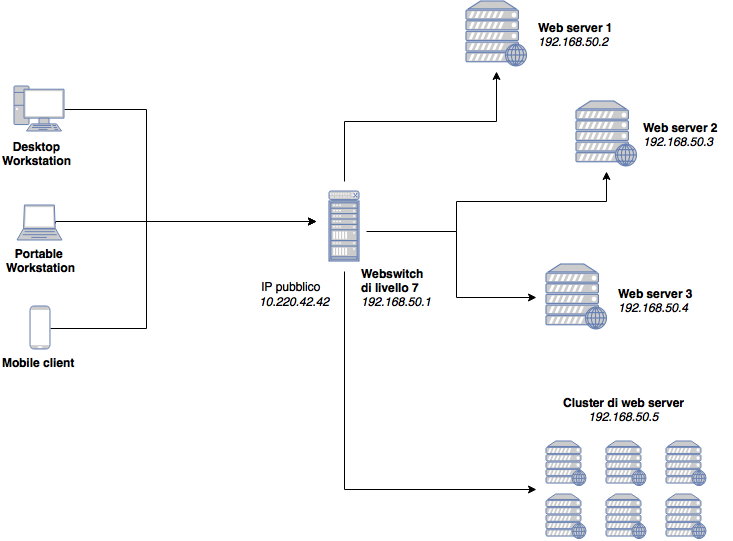
\includegraphics[width=\textwidth]{images/switch7}
\caption{Esempio di uno \emph{switch di livello 7 (OSI)}}
\end{figure}

\newpage
\section{Architettura}
\label{sec:architecture}


\subsection{Server in ascolto}
\label{sec:main}

\subsubsection{File di configurazione}
\label{sec:config}

\subsubsection{Logging}
\label{sec:logging}

\subsubsection{Gestione degli errori}
\label{sec:errors}

\subsection{Pool manager}
\label{sec:pool}

\subsection{Scheduler}
\label{ssec: sched}
Lo scheduler è un componente fondamentale di un sistema informatica: si occupa di stabilire un ordinamento temporale l'esecuzione di un set di richieste di accesso ad una risorsa. Nel caso di un web switch di livello 7, lo scheduler va a garantire che ognuna delle richieste in arrivo possa essere inoltrata immediatamente alla prima macchina disponibile, secondo una politica di scheduling che sia \emph{state-less}, quindi che non consideri l'attuale carico di lavoro delle macchine del cluster, oppure \emph{state-aware}, che monitori costantemente tale carico e modifichi di conseguenza l'assegnazione delle richieste (verrà spiegato nel dettaglio come lavorano e quando sono disponibili tali politiche in \emph{\ref{sec: sched_p}}). \\\\
In questa implementazione lo scheduler, che come vedremo va a sfruttare un algoritmo di selezione \emph{Round Robin} la cui struttura verrà esplicitata più avanti, viene definito come segue.
\begin{lstlisting}
/*
 * ---------------------------------------------------------------------------
 * Structure        : typedef struct scheduler_args
 * Description      : This struct represents the arguments necessary to run the
 *                    scheduler properly
 * ---------------------------------------------------------------------------
 */
typedef struct scheduler_args {
    RRobinPtr     rrobin;                                   // Round Robin struct
    ServerPoolPtr server_pool;                              // Server Pool struct

    ServerPtr (*get_server)(RRobinPtr rrobin);              // to retrieve a server
} Scheduler, *SchedulerPtr;


\end{lstlisting}
In particolare la \textbf{pool dei server} altro non è che un \emph{lista collegata} formata da strutture dati elementari per la gestione dei server indicati nel file di configurazione come appartenenti al cluster, definite come segue
\begin{lstlisting}
/* ---------------------------------------------------------------------------
 * Structure        : typedef struct server_node
 * Description      : This struct represents a single server node in order to
 *                    manage a pool of remote machines
 * ---------------------------------------------------------------------------
 */
typedef struct server_node {
    char *host_address;                                         // machine canonical name
    char *host_ip;                                              // machine ip address
    int  status;                                                // machine status
    int  weight;                                                // machine weight

    struct server_node *next;                                   // next server_node
} ServerNode, *ServerNodePtr;

\end{lstlisting}
mentre le strutture dati che vengono elaborate ed utilizzate come valore di ritorno della schedulazione e che sono alla base della costituzione del buffer su cui opera Round Robin, non sono altro che una versione semplificata e costituita dalle sole informazioni di base per la connessione. \\\\
Nella \textbf{fase di inizializzazione} viene quindi popolata la pool recuperando gli indirizzi delle macchine del cluster, che vengono settate come disponibili e con peso minimo. Quindi a seconda che si sia configurato il web switch in modalità \emph{state-aware} o \emph{state-less}, rispettivamente viene o non viene istanziato un thread che si occuperà di aggiornare periodicamente, con gestione degli accessi concorrenti al buffer del Round Robin, lo stato delle macchine. Ogni volta che una connessione viene accettata viene recuperato un server valido da passare al processo che gestirà la connessione tramite memoria condivisa. Lo scheduler è recuperabile tramite un \emph{singleton}.
\begin{lstlisting}
\* inside thread_pool.c ... *\
// Retrieving server from scheduler
ServerPtr server = get_scheduler()->get_server(get_scheduler()->rrobin);
// Storing server in shared memory
worker_pool->worker_server[position] = *server;
	
\end{lstlisting}
Viene sempre selezionato un server che sia disponibile, quindi viene sempre effettuato un controllo sullo \emph{status} dello stesso server, nel caso in cui sia abilitato il controllo sullo stato della macchina: l'unico caso in cui questi risulta \emph{BROKEN} e non \emph{READY} è nella circostanza in cui ogni server del cluster risulta non disponibile per cui il worker (che analizzeremo in \emph{\ref{sec:worker}}) non avvierà nessuna connessione di inoltro della richiesta. \\\\
Dalla necessità progettuale di garantire uno \textbf{scheduling adattabile} a condizioni di stress da carico, quindi per soddisfare specifiche di \emph{state-awareness}, nascono i parametri relativi a status e peso nei nodi della pool di server e nasce un adattamento \emph{pesato} dell'algoritmo di Round Robin. \\

\subsection{Worker}
\label{sec:worker}
Il \textbf{worker} è il componente principale di Heimdall e non a caso gli è stato assegnato questo nome poiché è lui che ``lavora'' andando a servire le richieste dei client tramite lo smistamento ai vari server presenti nel cluster e il successivo inoltro delle risposte.
\\
Nell'attuale implementazione il worker è un processo composto da quattro thread: il \hyperref[sec:reader]{\emph{thread di lettura}}, il \hyperref[sec:writer]{\emph{thread di scrittura}}, il \hyperref[sec:request]{\emph{thread di richiesta}} e il \hyperref[sec:watchdog]{\emph{thread di watchdog}}.
\\
Heimdall è configurato in modo tale da effettuare il \textbf{prefork} di un numero configurabile di processi (si veda \ref{sec:config}), questa scelta è stata fatta per evitare di aggiungere ritardo causato dal tempo di creazione di quest'ultimi.

\subsubsection{Gestione delle richieste}
\label{sec:requests_management}

% TODO biblio to HTTP1.1 https://tools.ietf.org/html/rfc2616#page-44
L'applicazione soddisfa le specifiche \textbf{HTTP 1.1} gestendo \textbf{connessioni persistenti} e supportando il \textbf{pipelining} delle richieste. Per ottenere il supporto alle connessioni persistenti Heimdall chiude la connessione con il client solo allo scadere di un timer, così facendo può ricevere più richieste tramite la stessa connessione. Queste non appena ricevute vengono inserite in una coda per essere poi servite nello stesso ordine con cui sono state ricevute.
Il worker è un processo che viene creato tramite prefork al primo avvio del WebSwitch. Questo rimane in pausa finché non gli viene consegnata una connessione da cui poter ricevere le richieste. Tale passaggio è realizzato tramite il \hyperref[sec:pool]{\emph{pool manager}} e in particolare dal message controller. Non appena ricevuta una connessione da poter servire, inizierà a lavorare creando i vari thread necessari per: la ricezione, l'inoltro e la successiva risposta alla richiesta.

\subsubsection*{Coda delle richieste}
\label{sec:requests_queue}

Come detto pocanzi per poter supportare il pipeling è stato necessario creare una coda che contenesse tutte le richieste effettuate da un client tramite la stessa connessione HTTP. È stata implementata una coda poiché è necessario rispettare l'ordine delle richieste all'atto della risposta.
% A server MUST send its responses to those requests in the same order that the requests were received. https://tools.ietf.org/html/rfc2616#section-8.1.2.2

La coda è molto semplice ed espone le seguenti operazioni:
\begin{lstlisting}
    void (*enqueue)(struct request_queue *self, RequestNodePtr node);
    struct request_node*(*dequeue)(struct request_queue *self);
    int (*is_empty)(struct request_queue *self);
    struct request_node*(*get_front)(struct request_queue *self);
    int (*get_size)(struct request_queue *self);

    void (*destroy)(struct request_queue *self);
\end{lstlisting}

Questa contiene elementi di tipo RequestNode, struttura dati che incapsula: la richiesta, la risposta, un riferimento al nodo precedente, al nodo successivo e, oltre altre variabili di supporto per il multithreading e per il watchdog, un'ulteriore struttura, il chunk.

\begin{lstlisting}
    pthread_t thread_id;
    HTTPRequestPtr request;
    HTTPResponsePtr response;
    time_t request_timeout;
    struct request_node *previous;
    struct request_node *next;
    ChunkPtr chunk;
    int *worker_status;
    pthread_mutex_t mutex;
    pthread_cond_t condition;
\end{lstlisting}

\subsubsection*{Chunk di dati}
\label{sec:chunk}
Un chunk è un ``pezzo'' che contiene parte della risposta. Questa scelta è stata adottata poiché si è preferito rispondere il più presto possibile al client senza dover attendere necessariamente di aver ottenuto la risposta completa poiché questa potrebbe essere corposa e quindi, oltre occupare ``molto'' spazio, potrebbe richiedere molto tempo per essere completamente ricevuta da Heimdall e aggiungerebbe solo ritardo per il seguente inoltro.
\\
La struttura è molto semplice e contiene un'area di memoria fissa allocata alla creazione del chunk di dimensione pari a 4096 byte.
\\
È stata fatta questa scelta per alleggerire al massimo il carico su Heimdall, in questo modo, non dovrà avere in memoria risposte complete ma facendo da ``passa carta'' tra server e client avrà in memoria in ogni istante il minor quantitativo di risorsa possibile. Questa implementazione è stata possibile grazie alla natura delle connessioni TCP, cioè quello di essere full duplex
% A connection can be used to carry data in both directions, that is, it is "full duplex".  https://tools.ietf.org/html/rfc793#section-2.7

% disegnino socket con tubicini che non venivano usati contemporaneamente se non fosse stato usato il chunk -  utilizzo socket con chunck
\subsubsection{Gestione delle connessioni}
\subsubsection*{Connessione}
Il sistema è stato concepito per essere il più modulare possibile con valori di ritorno il più possibile uniformi. La gestione delle connessioni ne è un esempio lampante. Abbiamo realizzato un wrapping delle API Socket di Berkley in modo tale da gestire tutti gli errori allo stesso modo, tramite l'utilizzo dei Throwable (si veda \ref{sec:errors}). Oltre a questo abbiamo, fin dove possible, cercato di rendere più snella l'implementazione delle chiamate in modo tale da poterci preoccupare solo della logica dell'applicazione e non dalla sua effettiva implementazione. Sono esplicative le funzioni per creare una nuova connessione di tipo server:
\begin{lstlisting}
/*
 * Function    : create_server_socket
 * Description : This function creates a TCP or a UDP server
 *               bound at specified port.
 *
 * Param       :
 *   type   : The type of the socket, 0 for TCP, 1 per UDP.
 *   port   : The number of the port where bind the server.
 *   sockfd : The pointer of the int where save the file
 *            description.
 *
 * Return      : A Throwable.
 */
ThrowablePtr create_server_socket(const int type, const int port, int *sockfd) {

    ThrowablePtr throwable = create_socket(type, sockfd);
    if (throwable->is_an_error(throwable)) {
        return throwable->thrown(throwable, "create_server_socket");
    }

    struct sockaddr_in addr;

    memset((void *) &addr, 0, sizeof(addr));    // Set all memory to 0
    addr.sin_family = AF_INET;                  // Set IPV4 family
    addr.sin_addr.s_addr = htonl(INADDR_ANY);   // Waiting a connection on all server's IP addresses
    addr.sin_port = htons(port);                // Waiting a connection on PORT

    if (bind(*sockfd, (struct sockaddr *) &addr, sizeof(addr)) == -1) {
        return get_throwable()->create(STATUS_ERROR, get_error_by_errno(errno), "create_server_socket");
    }

    return get_throwable()->create(STATUS_OK, NULL, "create_server_socket");
}
\end{lstlisting}

e di tipo client:
\begin{lstlisting}
/*
 * Function    : create_client_socket
 * Description : This function creates a TCP or a UDP client
 *              that connects itself at specific IP thorough
 *              a specific port.
 *
 * Param       :
 *   type   : The type of the socket, 0 for TCP, 1 per UDP.
 *   port   : The number of the port where bind the server.
 *   sockfd : The pointer of the int where save the file
 *            description.
 *
 * Return      : A Throwable.
 */
ThrowablePtr create_client_socket(const int type, const char *ip, const int port, int *sockfd) {

    ThrowablePtr throwable = create_socket(type, sockfd);
    if (throwable->is_an_error(throwable)) {
        return throwable->thrown(throwable, "create_client_socket");
    }

    struct sockaddr_in addr;

    memset((void *) &addr, 0, sizeof(addr));            // Set all memory to 0
    addr.sin_family = AF_INET;                          // Set IPV4 family
    addr.sin_port = (in_port_t) htons((uint16_t) port); // Set server connection on specified PORT

    if (inet_pton(AF_INET, ip, &addr.sin_addr) == -1) {
        return get_throwable()->create(STATUS_ERROR, get_error_by_errno(errno), "create_client_socket");
    }

    if (connect(*sockfd, (struct sockaddr *) &addr, sizeof(addr)) == -1) {
        return get_throwable()->create(STATUS_ERROR, get_error_by_errno(errno), "create_client_socket");
    }

    return get_throwable()->create(STATUS_OK, NULL, "create_client_socket");
}
\end{lstlisting}
Questo approccio ci ha permesso per esempio di modificare più volte il codice che permetteva l'invio delle richieste e la ricezione delle risposte, senza andare a stravolgere, per quanto possibile, la logica del sistema.
% TODO RFC reference in (**)
\subsubsection*{Richieste HTTP}
Alla base della capacità del web switch di inoltrare ad una macchina del cluster la richiesta che gli viene effettuata dal client, vi è la capacità di poter analizzare tale richiesta e poterne trarre le corrette informazioni. \\
Per questo sono state definite macro degli \emph{header} più importanti come da (**) per poter \emph{parsare} il pacchetto HTTP una volta che questo è correttamente giunto (completo) al web switch. E' stata quindi definita la struct seguente.
\begin{lstlisting}
/*
 * ---------------------------------------------------------------------------
 * Structure        : typedef struct http_request
 * Description      : This struct collect all attributes and functions pointers to
 *                    manage, retrieving or creating, HTTP requests
 * ---------------------------------------------------------------------------
 */
typedef struct http_request {
    char *status;                                       // whether the request can be handled
    char *req_type;                                     // type of the request
    char *req_protocol;                                 // accepted only HTTP/1.1
    char *resp_code;
    char *resp_msg;
    char *req_resource;                                 // resource locator
    char *req_accept;                                   // accepting content info
    char *req_from;                                     // client and request generic info
    char *req_host;
    char *req_content_type;                             // content type info
    int   req_content_len;
    char *req_upgrade;                                  // no protocol upgrade are allowed

    char *header;                                

    ThrowablePtr (*get_header)(struct http_request *self, char *req_line);
    ThrowablePtr (*get_request)(struct http_request *self, char *req_line, int len);
    ThrowablePtr (*read_headers)(struct http_request *self, char *string, int type);
    ThrowablePtr (*make_simple_request)(struct http_request *self, char **result);
    ThrowablePtr (*set_simple_request)(struct http_request *self, char *request_type, char *request_resource, char *request_protocol, char *host);
    void (*destroy)(struct http_request *self);
} HTTPRequest, *HTTPRequestPtr;

\end{lstlisting}
Per cui una volta inizializzata può essere utilizzata per memorizzare, attraverso la lettura degli \emph{header} e dei parametri ad essi associati le informazioni necessarie per poter inoltrare alla macchina del cluster selezionata. Sono state utilizzate le convenzioni previste del protocollo già viste nell'RFC precedentemente indicato: in particolare la corretta lettura di \emph{<carriage return><newline>} singolo e doppio rispettivamente a fine riga e come separatore fra headers e contenuto del pacchetto, per poter determinare gli estremi di lettura del \emph{parser}. \\ 
Osserviamo come non siano presenti tutti gli header definiti dal protocollo e come alcuni siano definiti per quanto riguarda la risposta HTTP (su questo aspetto torneremo fra poco). \\\\
Particolarmente importanti per questa implementazione sono i parametri che definiscono \emph{tipo di richiesta}, \emph{protocollo} e \emph{risorsa richiesta}. All'interno della struct è altresì presente un set di puntatori a funzione che consente di impostare i parametri per costruire una semplice richiesta HTTP, funzionalità che viene usata per inoltrare la richiesta al cluster.
\subsubsection*{Risposte HTTP}
La modularità della struct vista per quanto riguarda l'analisi della richiesta HTTP ha consentito di includere in essa anche i parametri, come il \emph{messaggio ed il codice di risposta}, nonchè la \emph{lunghezza della risorsa} contenuta nel pacchetto, necessari per la corretta lettura di un completo pacchetto HTTP di risposta. Per cui è bastato utilizzare le funzionalità già implementata ed "estendere" la struttura precedente come segue.
\begin{lstlisting}
	/*
 * ---------------------------------------------------------------------------
 * Structure        : typedef struct http_response
 * Description      : This struct collect all attributes and functions pointers to
 *                    manage, retrieving or creating, HTTP responses
 * ---------------------------------------------------------------------------
 */
typedef struct http_response {
    struct http_request  *response;                           
    int    http_response_type;                                 
    char  *http_response_body;                                 // the body of the message

    ThrowablePtr (*get_http_response)(struct http_response *self, char *buffer);
    ThrowablePtr (*get_response_head)(struct http_response *self, char *head);
    ThrowablePtr (*get_response_body)(struct http_response *self, char *body);
    void (*destroy)(struct http_response *self);
} HTTPResponse, *HTTPResponsePtr;

\end{lstlisting}
L'unica differenza con l'implementazione già descritta è il mantenimento in un'area di memoria dell'originale contenuto del pacchetto inviato dal server, necessario per poter correttamente inoltrare al client la risposta senza dover rilavorare anche con il contenuto della risposta HTTP. Questo ha portato ad una riduzione dell'overhead soprattutto in condizioni in cui tale contenuto è un file di testo consistente od un'immagine.

\subsubsection{Thread di lettura}
\label{sec:reader}
Il thread di lettura ha il compito di leggere le richieste dalla socket tramite una read bloccate una volta che il worker ha ricevuto una connessione da gestire. Quindi accoda le richieste del client, per un massimo numero di richieste configurabile (si veda \ref{sec:config}) andando a creare per ogni richiesta un thread di richiesta che, dialogando con un server nella pool, si occuperà di gestirla. Il thread di lettura quindi è bloccato costantemente in attesa di nuove richieste e, ogni qual volta riceve una nuova connessione, aggiorna un timer adibito alla verifica dello stato di vita della connessione (si veda il paragrafo \ref{sec:watchdog}).
\begin{lstlisting}
// Gets queue
RequestQueuePtr queue = worker->requests_queue;

while (TRUE) {
    // Waits
    while (max_thr_request > 100) {
      if (pthread_cond_wait(&cond_thr_request, &mtx_thr_request) != 0) {
        return get_throwable()->create(STATUS_ERROR, get_error_by_errno(errno), "receive_http_chunks");
      }
    }

    // Updates timer
    worker->watchdog->timestamp_worker = time(NULL);

    // Creates the node
    RequestNodePtr node = init_request_node();
    if (node == NULL) {
      get_log()->e(TAG_WORKER, "Malloc error in init_request_node");
      worker->reader_thread_status = STATUS_ERROR;
      return NULL;
    }
    node->worker_status = &worker->request_thread_status;

    // Enques the new node
    queue->enqueue(queue, node);

    // Receives request
    ThrowablePtr throwable = receive_http_request(worker->sockfd, node->request);
    if (throwable->is_an_error(throwable)) {

      get_log()->t(throwable);
      worker->reader_thread_status = STATUS_ERROR;

      // if we get some error on cliebt socket
      worker->worker_await_flag = WATCH_OVER;
      pthread_cond_signal(&worker->await_cond);

      pthread_exit(NULL);
    }

    request_counter++;

    // Creates the request thread
    int request_creation = pthread_create(&(node->thread_id), NULL, request_work, (void *) node);
    if (request_creation != 0) {
      get_log()->t(get_throwable()->create(STATUS_ERROR, get_error_by_errno(errno), "read_work"));
      worker->reader_thread_status = STATUS_ERROR;
      return NULL;
    }

    // Gets mutex
    if (pthread_mutex_lock(&mtx_thr_request) != 0) {
      return get_throwable()->create(STATUS_ERROR, get_error_by_errno(errno), "receive_http_chunks");
    }

    max_thr_request++;

    // Sends signal to condition
    if (pthread_cond_signal(&cond_thr_request) != 0) {
      return get_throwable()->create(STATUS_ERROR, get_error_by_errno(errno), "receive_http_chunks");
    }

    // Releases mutex
    if (pthread_mutex_unlock(&mtx_thr_request) != 0) {
      return get_throwable()->create(STATUS_ERROR, get_error_by_errno(errno), "receive_http_chunks");
    }
}
\end{lstlisting}

\subsubsection{Thread di scrittura}
\label{sec:writer}
Il thread di scrittura è adibito all'inoltro della risposta ottenuta tramite il \hyperref[sec:request]{\emph{thread di richiesta}}. Questi due thread cooperano per mezzo di una condition andando a scrivere e a leggere nella stessa area di memoria, il \hyperref[sec:chunk]{\emph{chunk}}. Dovendo rispondere in ordine il thread si trova in loop sulla coda delle richieste andando a richidere sempre il fronte di questa e, dopo aver inviato l'header di risposta (che non è gestito tramite chuck), inizia questo ``balletto'' con il \hyperref[sec:request]{\emph{thread di richiesta}}.
\begin{lstlisting}
// Gets queue
RequestQueuePtr queue = worker->requests_queue;

while(TRUE) {

    // Gets node
    RequestNodePtr node = queue->get_front(queue);

    if (node != NULL) {

        // Gets mutex
        if (pthread_mutex_lock(&node->mutex) != 0) {
            get_log()->t(get_throwable()->create(STATUS_ERROR, get_error_by_errno(errno), "write_work"));
            worker->writer_thread_status = STATUS_ERROR;
            return NULL;
        }

        while (node->response->response->header == NULL) {
            if (pthread_cond_wait(&node->condition, &node->mutex) != 0) {
                get_log()->t(get_throwable()->create(STATUS_ERROR, get_error_by_errno(errno), "write_work"));
                worker->writer_thread_status = STATUS_ERROR;
                return NULL;
            }
        }

        // Sends the response header
        ThrowablePtr throwable = send_http_response_header(worker->sockfd, node->response);
        if (throwable->is_an_error(throwable)) {
            get_log()->t(throwable);
            worker->writer_thread_status = STATUS_ERROR;

            // unlock if error
            if (pthread_mutex_unlock(&node->mutex) != 0) {
                get_log()->t(get_throwable()->create(STATUS_ERROR, get_error_by_errno(errno), "write_work"));
            }

            return NULL;
        }

        // Releases mutex
        if (pthread_mutex_unlock(&node->mutex) != 0) {
            get_log()->t(get_throwable()->create(STATUS_ERROR, get_error_by_errno(errno), "write_work"));
            worker->writer_thread_status = STATUS_ERROR;
            return NULL;
        }

        // Gets the chunk
        ChunkPtr chunk = node->chunk;

        // Sends the response chunks
        throwable = send_http_chunks(worker->sockfd, chunk, node->response->response->req_content_len);
        if (throwable->is_an_error(throwable)) {
            get_log()->t(throwable);
            worker->writer_thread_status = STATUS_ERROR;
            return NULL;
        }

        // Dequeues the request and it destroys that
        node = queue->dequeue(queue);
        node->destroy(node);
    }
}
\end{lstlisting}

\subsubsection{Thread di richiesta}
\label{sec:request}
Il thread di richiesta è adibito infine all'invio della richiesta ad un server nel cluster e alla successiva 
\subsubsection{Thread di watchdog}
\label{sec:watchdog}
\begin{figure}[h]
\centering
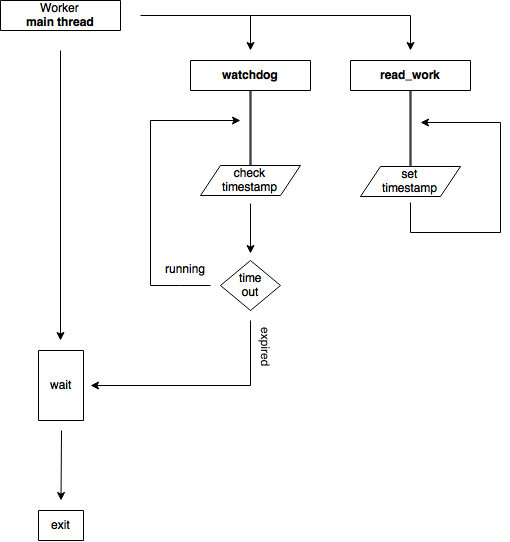
\includegraphics[width=\textwidth]{images/watchdog}
\caption{Schema della procedura di controllo sul tempo di esecuzione \label{fig: watchdog}}
\end{figure}
Il thread di \emph{watchdog}, letteralmente di sorveglianza, è adibito al controllo della \textbf{corretta esecuzione del worker},in particolare al controllo che tale esecuzione, nell'occupare per eccessivo tempo le risorse del sistema, non vado a creare un collo di bottiglia che via via porta al collasso del programma. Per far questo esso viene eseguito in modalità \emph{detached} dal thread principale del worker ed è legato dalle operazioni che vengono eseguite dal processo da una serie di variabili: 
\begin{itemize}
	\item \emph{pthread\_condition} su cui è in attesa il thread principale del worker
	\item \emph{flag} legata alla condition di cui sopra
	\item \emph{timestamp} settato dal thread di lettura della richiesta in arrivo
\end{itemize}
Come appare da una prima analisi della struct del watchdog.
\begin{lstlisting}
/*
 * ---------------------------------------------------------------------------
 * Structure        : typedef struct watchdog_thread
 * Description      : this struct helps to manage and set attributes for the thread
 *                    which watch over the remote connection thread termination
 * ---------------------------------------------------------------------------
 */
typedef struct watchdog_thread {
    int status;                                     
    pthread_cond_t *worker_await_cond;             
    int *worker_await_flag;

    time_t killer_time;                             // to schedule the watchdog wakeup
    time_t timeout_worker;                          // to abort a thread run
    time_t timestamp_worker;                        // timestamp last worker operation
} Watchdog, *WatchdogPtr;

\end{lstlisting}
Dove il \emph{killer\_time} ed il \emph{timeout\_worker} sono definiti dal file di configurazione per dare modo all'operatore di modellare l'implementazione sulle caratteristiche della macchina su cui gira il web switch. \\\\
Una più schematica rappresentazione del flusso di esecuzione è possibile vederla in \emph{\ref{fig: watchdog}}.
In particolare quando vengono distaccati i thread ausiliari, il thread principale del worker si mette in attesa della fine di una delle condizioni di termine del servizio di cui si è già discusso sopra, fra cui anche lo scadere del massimo tempo di esecuzione disponibile. In particolare, ad ogni iterazione del thread di lettura, avremo un aggiornamento del timestamp del worker, per cui ogni volta che si ha l'arrivo di una risposta da reinoltrare o di una richiesta da soddisfare si assume il server come operativo od il client in ascolto. \\ 
Contemporaneamente il watchdog rimane in \emph{nanosleep} per un lasso di tempo pari a quello configurato, a meno dell'arrivo di segnali che vengono gestiti e dopo i quali il watchdog ritorna in attesa, scaduto il quale la variabile di timestamp viene controllata. Se risulta \emph{scaduta} viene aggiornato il flag di attesa del worker e gli viene segnalato di riattivarsi e di mettere in pratica le procedure di \emph{clean up} per scollegarsi dal client e dal server assegnato. \\\\
Osserviamo come questo controllo viene fatto su una variabile settata dal thread di lettura, permettendoci con semplicità di valutare eventuali problemi sia sulla linea fra web switch e macchina del cluster che fra web switch e client, evitando lo stato di \emph{hanging} che porterebbe ad uno stallo del programma.
\newpage
\section{Ulteriori proposte}

\newpage
\section{Politiche di scheduling}
 \label{sec: sched_p}
La schedulazione permette la selezione della macchina predisposta a rispondere alla richiesta HTTP appena arrivata da parte del client, si basa su una tecnica nota come \textbf{bilanciamento del carico}, ovvero la distribuzione del carico, solitamente di elaborazione o di erogazione di uno specifico servizio, tra più server. Questo permette di poter \textbf{scalare} sulla potenza di calcolo del cluster dietro al web switch, lasciando che siano diverse macchine a rispondere a seconda di quella che è più veloce, più performante, oppure monitorando costantemente lo stato dei server e scegliendo quello meno sottoposto ad una pressione del carico di lavoro. Le macchine, specificando hostname ed indirizzi IP, sono date in un apposito file di configurazione.
\\
\\
Nella nostra implementazione \textbf{thread scheduler} si occupa di fornire,  ogni volta che viene invocato, una macchina selezionata secondo una delle due politiche che andremo ora a spiegare nel dettaglio.

\subsection{State-less: implementazione con Round-Robin}
L'algoritmo di scheduling Round-Robin (da adesso RR, \emph{n.d.r.}) è un algoritmo che agisce con prelazione distribuendo in maniera equa il lavoro, secondo una metrica stabilita in partenza. Vediamo quindi la struttura che si occupa di gestire la schedulazione tramite Round-Robin e che contiene le funzioni \emph{wrapper} alle strutture dati che garantiscono il suo corretto funzionamento.\\
\begin{lstlisting}
/*
 * ---------------------------------------------------------------------------
 * Structure        : typedef struct round_robin_struct
 * Description      : This struct represents a Round Robin discipline that can
 *                     be used also a stateful discipline with minimum overhead
 *                    (weighted mode enabled)
 * ---------------------------------------------------------------------------
 */
typedef struct round_robin_struct {
    CircularPtr circular;

    ThrowablePtr (*weight)(CircularPtr circular, Server *servers, int server_num);
    ThrowablePtr (*reset)(RRobinPtr rrobin, ServerPoolPtr pool, int server_num);
    Server *(*get_server)(CircularPtr circular);
}RRobin, *RRobinPtr;

\end{lstlisting}
\begin{figure}[b]
\centering
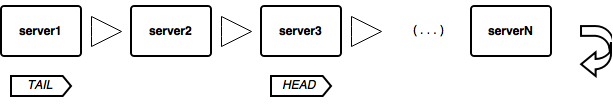
\includegraphics[width=\textwidth]{images/rrobin_stateless}
\caption{Schema di funzionamento del buffer circolare \label{fig: rrobin_sl}}
\end{figure}
Possiamo osservare come siano mantenuti i puntatori alle funzioni necessarie al caso di politica di scheduling \emph{state-aware}, ma per ora l'unica vera funziona a cui si farà accesso è quella per il recupero del server correntemente selezionato. \\\\
L'algoritmo funziona utilizzando un \textbf{buffer circolare} come possiamo vedere in \emph{figura \ref{fig: rrobin_sl}}: questo permette di iterare la selezione su una lista di elementi precedentemente caricata. Possiamo osservare che, oltre alle funzioni e le variabili necessarie a garantire l'accesso atomico all'area di memoria che contiene il buffer, necessario come vedremo nel caso \emph{state-aware} per evitare la concorrenza con il thread che si occupa dell'update dello stato, sono mantenuti:
	\begin{itemize}
  		\item Un puntatore all'array di server 
  		\item La posizione attuale del puntatore di \emph{testa} 
  		\item La lunghezza del buffer, necessaria anche per le operazioni di aggiornamento dei puntatori
  		\item I puntatori di \emph{testa} e \emph{coda} per avanzamento e lettura dal buffer
	\end{itemize}
	Le funzioni restanti permettono di inizializzare il buffer (oltre che di liberare con sicurezza l'area di memoria occupata) e di aggiornare i puntatori sopra menzionati.\\

\subsection{State-less: implementazione con Round-Robin}
L'algoritmo di scheduling Round-Robin (da adesso RR, \emph{n.d.r.}) è un algoritmo che agisce con prelazione distribuendo in maniera equa il lavoro, secondo una metrica stabilita in partenza.
\\
L'algoritmo funziona utilizzando un buffer circolare come possiamo vedere in \hyperref[fig: rrobin_sl]{\emph{figura}}: questo permette di iterare la selezione su una lista di elementi precedentemente caricata. E' necessario quindi specificare due passi per il corretto funzionamento, dopo aver dato un rapido sguardo alla struttura che lo rappresenta nella nostra implementazione.
\\
\\
\begin{lstlisting}
/*
 * ---------------------------------------------------------------------------
 * Structure        : typedef struct circular_buffer
 * Description      : This struct helps to manage a circular buffer of fixed length
 * ---------------------------------------------------------------------------
 */
typedef struct circular_buffer {
    Server      *buffer;
    int         buffer_position;
    int         buffer_len;
    
    Server      *head;
    Server      *tail;

    pthread_mutex_t mutex;

    ThrowablePtr (*allocate_buffer)(CircularPtr *circular, Server **servers, int len);
    ThrowablePtr (*acquire)(struct circular_buffer *circular);
    ThrowablePtr (*release)(struct circular_buffer *circular);
    void         (*progress)(struct circular_buffer *circular);
    void         (*destroy_buffer)(struct circular_buffer *circular);
} Circular, *CircularPtr;

\end{lstlisting}
\break
È necessario quindi specificare tre passi per il corretto funzionamento, dopo aver dato un rapido sguardo alla struttura che lo rappresenta nella nostra implementazione. \\\\
\textbf{Inizializzazione del buffer} in questa fase la struttura dati che rappresenta il buffer circolare, che abbiamo visto mantenere due puntatori di \emph{testa} e \emph{coda}, viene inizializzata associandovi un array di puntatori di strutture di tipo \emph{Server}, precedentemente allocata ed il cui pattern è stato fissato, e viene eseguita la funzione di allocazione del buffer: 
\begin{lstlisting}
    /* inside allocate_buffer ... */
    // allocating the buffer
    circular->buffer = *servers;
    circular->buffer_len = len;
    // setting params
    circular->head = circular->buffer;
    circular->tail = circular->buffer + (len - 1);
    
\end{lstlisting}
In un'ottica di \emph{produttore vs consumatore}, chiaramente visibile nella figura precedente, è necessario che testa e coda non coincidano mai per evitare concorrenza. In questa implementazione si è deciso di separare l'accesso concorrente alla struttura, per il suo aggiornamento, e la lettura dei dati in essa contenuti. Quindi la \emph{testa} conterrà il puntatore al prossimo server da selezionare per schedulare la richiesta, mentre la \emph{coda} punterà all'area di memoria contenente il server attualmente selezione per la schedulazione. \\\\
\textbf{Aggiornamento dei puntatori} per poter sfruttare le peculiarità di questa struttura dati è necessario che i due puntatori vengano aggiornati secondo l'aritmetica del buffer circolare per cui, una volta raggiunta l'estremità dell'array, il valore successivo della posizione corrente ritorna ad essere quello del primo valore dello stesso array. \\
Nel dettaglio viene eseguito, secondo le specifiche sopra riportate, nella nostra implementazione, la seguente funzione:
\begin{lstlisting}
void progress(CircularPtr circular) {
    // recomputing tail, head and buffer position
    circular->tail            = circular->head;
    circular->buffer_position = (circular->buffer_position + 1) % circular->buffer_len;
    circular->head            = circular->buffer + circular->buffer_position;
}

\end{lstlisting}
\textbf{Selezione del server} a questo punto, una volta che il thread chiamante invoca lo scheduler per recuperare il server che è stato selezionato dall'algoritmo, lo scheduler a sua volta invoca la funzione wrapper dalla struttura che gestisce la politica RR e questa esegue il codice ora riportato.
\begin{lstlisting}
    /* inside get_server ... */
    // allocating server ready struct
    ServerPtr server_ready = malloc(sizeof(Server));
   
    /* ... */
    
    // stepping the circular buffer
    circular->progress(circular),
    // retrieving server from tail 
    *server_ready = *(circular->tail);
    return server_ready;
    
\end{lstlisting}
In conclusione quello che stiamo attuando è un \textbf{bilanciamento del carico uniforme} su ognuna delle macchine del cluster. Infatti, senza condizioni sullo stato delle macchine, iterando semplicemente sull'array dei server, ad ogni nuova connessione verrà assegnata una macchina diversa, alleggerendo tutti i server e pareggiando per ciascuno il carico. Il cluster manterrà il carico complessivo ma ogni singola unità contribuirà equamente a soddisfare le connessioni in arrivo.
\newpage
\subsection{State-aware: implementazione con monitor di carico}

\begin{figure}[t]
\centering
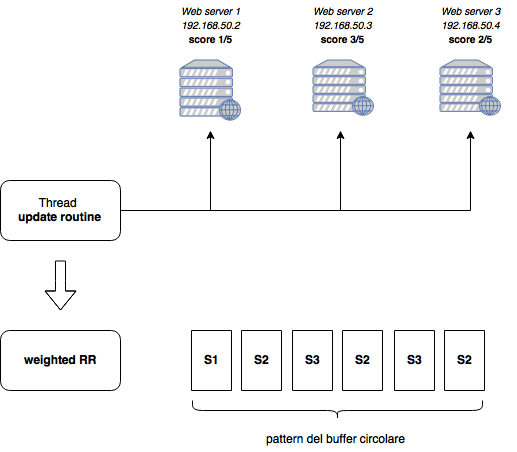
\includegraphics[width=\textwidth]{images/rrobin_stateaware}
\caption{Schema della procedura di aggiornamento dello stato dei server
\label{fig:rrobin_sa}}
\end{figure}

Un algoritmo di schedulazione cosiddetto \emph{state-aware} si occupa di selezionare la macchina a cui inoltrare la connessione basandosi non solo sulla conoscenza delle macchine presenti nel cluster ma anche sul loro status. In particolare, in questa implementazione, si è deciso di ricorrere all'analisi dei risultati di un \textbf{monitor di carico} presente su ciascuna delle macchine del cluster (in riferimento alle assunzioni progettuali, questi è i modulo \emph{ApacheStatus} di cui si parlerà più avanti in \emph{\ref{sssec:apachestatus}} ). Tale monitor, che ritorna una serie di parametri indici dell'attuale impiego di risorse della macchina, permette di definire un \textbf{algoritmo pesato} per la selezione del server che risponderà alla connessione in arrivo al web switch. \\
Anche in questo caso andremo a determinare una serie di passi che vengono seguiti, tenendo conto che in fase progettuale \emph{si è deciso di sfruttare lo stesso algoritmo RR} già utilizzato nel caso \emph{state-less}, ma che ricordiamo essere stato predisposto per una ulteriore versione pesata. Per far questo si lavora sulla struttura Server \\\\
\textbf{Detachment del thread di update} nei file di configurazione dell'applicazione è possibile definire due livelli di lavoro:
	\begin{itemize}
		\item \textbf{AWARENESS\_LEVEL\_LOW} che corrisponde ad una versione state-less dell'algoritmo RR e si riporta al caso precedente
		\item \textbf{AWARENESS\_LEVEL\_HIGH} che corrisponde all'algoritmo state-aware e che necessiterà di una routine di aggiornamento dello stato delle macchine del cluster
	\end{itemize}
	Il secondo caso è proprio quello qui descritto e corrisponde a lavorare utilizzando, oltre al thread principale che si occupa di accettare le connessioni in arrivo, un \textbf{thread predisposto alla sola verifica dello stato dei server}. Tale thread viene istanziato nel momento in cui viene inizializzato lo scheduler e vengono allocate le strutture dati alla base di RR. \\
	Il lavoro di tale thread, che ora vedremo nel dettaglio, è quello deducibile da \emph{figura \ref{fig:rrobin_sa}}.\\\\
\textbf{Routine di score} all'interno di questa routine, che viene eseguita da un thread distaccato e che viene eseguita una volta ogni \emph{UP\_TIME} secondi, tempo di update in secondi definito dall'utente nei file di configurazione, viene richiamata più volte la funzione che si occupa di recuperare e parsare l'interrogazione del modulo \emph{ApacheStatus} e recupare da questa i \textbf{worker in \emph{idle state} ed i worker in \emph{busy state}}. A questo punto si va a modificare il nodo della pool dei server precedentemente allocata (di cui si è già parlato in \emph{\ref{ssec: sched}}). Viene quindi eseguita la sequente routine. \\
\begin{lstlisting}
    /* inside apache_score ... */
    // retrieving status from remote Apache machine
    throwable = apache_status->retrieve(apache_status);   
    //checking for errors or if server is currently down
    if (throwable->is_an_error(throwable)) {
        server->weight = WEIGHT_DEFAULT;
        server->status = SERVER_STATUS_BROKEN;
        return throwable->thrown(throwable, "apache_score");
    } else {
        server->status = SERVER_STATUS_READY;
    }
    
    /* ... */
    int score;
    int IDLE_WORKERS  = apache_status->idle_workers;
    int TOTAL_WORKERS = apache_status->busy_workers + IDLE_WORKERS;

    // calculating and setting score - mapping in [w, W]
    score = (IDLE_WORKERS   - WEIGHT_DEFAULT)   *
            (WEIGHT_MAXIMUM - WEIGHT_DEFAULT)   /
            (TOTAL_WORKERS  - WEIGHT_DEFAULT)   +   WEIGHT_DEFAULT;
    server->weight = score;
       
\end{lstlisting}
Alla fine quello che ottengo è uno \textbf{score} che vado a settare nel nodo contenuto nella \textbf{pool dei server} che viene definito dalla relazione matematica che è così esplicitata:
\begin{align*}
	score\Big(\frac{IDLE\_WORKERS}{TOTAL\_WORKERS}\Big) ~ \in ~ [w, W]
\end{align*}
ottenendo quello che un \emph{mapping} del rapporto fra i worker occupati nella macchina ed i worker totali a disposizione di Apache per rispondere ad una richiesta in arriva. Tale indice viene memorizzato come \emph{peso del server nel cluster}.\\
Notiamo che nel caso ci siano problemi nel recuperare l'indice di score si supporrà che il server non è momentaneamente disponibile ed il suo status verrà segnalato come BROKEN, fino al prossimo aggiornamento.\\\\
\textbf{RR pesato} dai nodi della pool dei server aggiornati con il loro peso viene costruito, secondo lo schema in \emph{\ref{fig:rrobin_sa}}, un pattern dei server secondo il loro peso, di modo da distribuire il carico secondo sempre un algoritmo RR, ma in cui per ogni sequenza il server viene selezionato un numero di volte pari al suo peso: comparirà massimo \emph{W} in caso di basso carico di lavoro ed al minimo \emph{w} volte in condizioni di forte stress. I due parametri sono, in questa implementazione, macro che possono essere modificate a seconda dei limiti delle macchine del proprio cluster, di default \emph{w = 1} e \emph{W = 5}, soggetti al tuning del web switch in fase di installazione ed ottimizzazione. Alla prima iterazione tutte le macchine so di default settata con peso minimo (pari a \emph{w})\\\\
In conclusione, con questa opzione abilitata, si ha la possibilità di ridistribuire equamente il lavoro, permettendo al web switch di adattare la distribuzione del carico a secondo dello stato attuale, evitando di sovraccaricare nodi sensibili allo stress in determinate condizioni o che sono stati sottoposti già ad uno stress eccessivo. Si è scelto di riadattare RR per ottenere una soluzione modulare e che fosse facile riadattare ed ottimizzare a seconda di entrambe le condizioni operative, sia senza che con conoscenza dello stato delle macchine. Osserviamo infatti che in entrambi i casi RR risulta pesato, nel secondo caso preso in esame tale peso non è più fisso e minimo ma variabile dipendentemente dalle condizioni delle macchine.\\\\
La ricerca di una soluzione modulare che possa essere presa poi in esame da futuri sviluppatore e possa essere oggetto di un \emph{tuning} più approfondito, è stata intrapresa perseguendo il principio per cui \emph{simplicity favours regularity}.

\subsubsection{Modulo Apache Status}
\label{sssec:apachestatus}
Il modulo Apache Status (modstatus) è un modulo che fornisce informazioni sull'attività e le prestazioni del server in cui è installato. Questo modulo è disponibile nella versione base di Apache senza il bisogno di dover scaricare nient altro, per utilizzarlo è necessario solo attivarlo nella configurazione del sito. Il modulo formatta tramite una pagina HTML tutta una serie statistiche e dati facilmente leggibili da un essere umano (oppure nella sua variante machine readble che in questa applicazione usiamo). I dettagli che fornisce sono il numero di worker che servono richieste, il numero di worker che sono in pausa, lo stato di ognuno di questi worker, il numero di accessi e byte serviti, il numero di richieste per secondo e la percentuale di CPU usata da ogni worker e in totale da Apache.
Tramite questo modulo quindi siamo stati in grado di poter verificare lo stato di una macchina senza la necessità di installare nessun componente aggiuntivo.
\subsubsection{Performance della politica state aware}
E' interessante osservare l'effettivo lavoro dello scheduler e della politica di \emph{state awareness} già commentata, in una condizione di forte stress delle macchine, nell'estratto del file di log che segue. La situazione proposta è stata ottenuta sovraccaricando una delle macchina del cluster e lasciando che il web switch si accorgesse di tale sovraccarico per bilanciare le richieste in arrivo.

\begin{lstlisting}[basicstyle=\fontsize{6.4}{7}\selectfont\ttfamily]

[Wed Feb 10 11:31:44 2016] - 192.168.1.3 to: 192.168.1.4 - worker: 3032 - GET / HTTP/1.1
[Wed Feb 10 11:31:44 2016] - 192.168.1.3 to: 192.168.1.5 - worker: 3031 - GET / HTTP/1.1
[Wed Feb 10 11:31:45 2016] - 192.168.1.3 to: 192.168.1.6 - worker: 3040 - GET / HTTP/1.1
[Wed Feb 10 11:31:45 2016] - 192.168.1.3 to: 192.168.1.5 - worker: 3039 - GET / HTTP/1.1
[Wed Feb 10 11:31:45 2016] - 192.168.1.3 to: 192.168.1.6 - worker: 3038 - GET / HTTP/1.1
[Wed Feb 10 11:31:45 2016] - 192.168.1.3 to: 192.168.1.5 - worker: 3037 - GET / HTTP/1.1
[Wed Feb 10 11:31:45 2016] - 192.168.1.3 to: 192.168.1.6 - worker: 3036 - GET / HTTP/1.1
[Wed Feb 10 11:31:45 2016] - 192.168.1.3 to: 192.168.1.5 - worker: 3035 - GET / HTTP/1.1
[Wed Feb 10 11:31:45 2016] - 192.168.1.3 to: 192.168.1.6 - worker: 3034 - GET / HTTP/1.1
\end{lstlisting}
\begin{figure}[H]
\centering
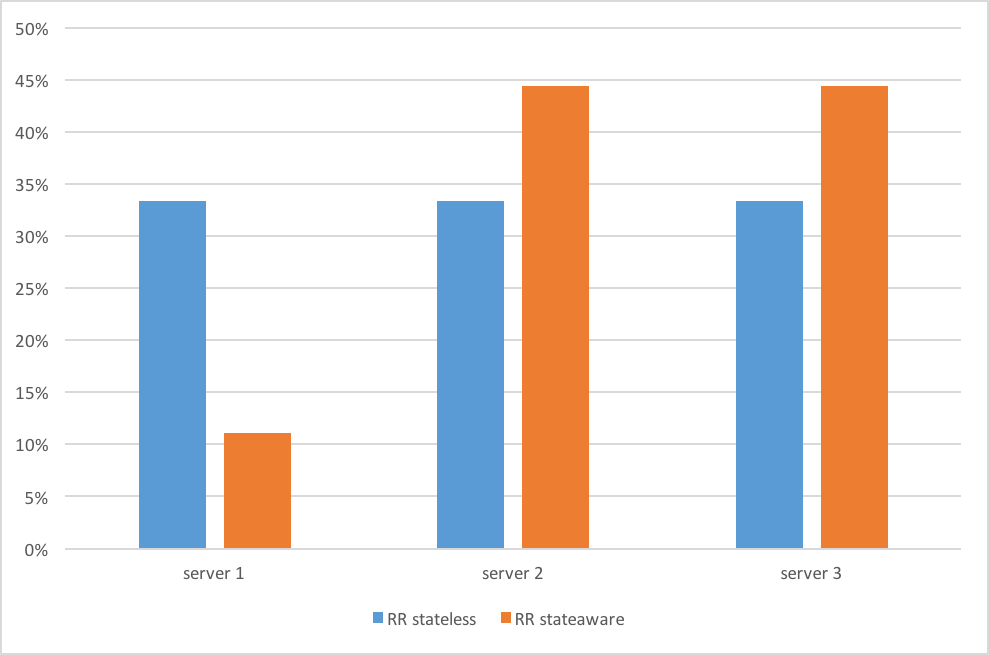
\includegraphics[width=\textwidth]{images/round_robin_cfr}
\caption{Ripartizione del carico di lavoro, \emph{confronto fra politica state-less e state-aware}\label{fig: rrobin_cfr}}
\end{figure}
In queste circostanze, considerato che secondo la nostra implementazione un server deve apparire almeno una volta nel buffer circolare, considerato che uno dei server era stato sottoposto a forte carico e che gli altri due server avevano un peso relativo superiore di tre unità, otteniamo che il server a venire meno sottoposto a connessioni in arrivo è proprio il server il cui carico di lavoro è già calcolato come particolarmente elevato. \\
E' possibile accertarlo sia dall'estratto del file di log riportato che alla \emph{\ref{fig: rrobin_cfr}} che ne quantifica i risultati.

\newpage
\section{Performance}
Abbiamo visto più volte durante questa trattazione che è stato necessario sottoporre a \emph{tuning} l'effettiva implementazione del server o che si consiglia di modellare quanti più aspetti possibili del web switch secondo la rete e le capacità della macchina. Riportiamo qui alcuni test che sono stati utilizzati in fase di progettazione per modellare la risposta del programma. I test sono stati condotti su:
	\begin{itemize}
		\item Macchina virtuale con Ubuntu Server 15.10 - 512 MB di RAM 
		\item Macchina con Ubuntu Desktop 15.10 - 6 GB di RAM, processore Intel i3 (1,9 GHz) 	
	\end{itemize}
Nel primo caso durante tutta la fase di sviluppo, nel secondo caso durante i test di carico per dare possibilità al web switch di non dover dipendere dall'hardware virtualizzato. Consideremo in tutti i casi la rete non saturata, in particolare non consideriamo la possibilità di influenze da parte di traffico generato da altre fonti essendo i test, per necessità, condotti o con una rete locale fra macchine collegate da uno switch di rete, oppure in locale su diverse macchine virtuali. \\\\ 
\textbf{Numero di processi e limite dei file descriptor} durante i test che seguono il numero di worker, variabile nelle configurazioni, è fissato a 10 come di default. Questo è stato giustificato da un'osservazione in fase sperimentale: non esiste una vera e propria variazione apprezzabile delle performance all'aumentare del numero di worker sopra i 10-15. Il valore di 10 unità è stato proposto per evitare sia un eccessivo utilizzo della memoria, sia per limitare il lavoro complessivo durante la creazione dei thread, sia per evitare ulteriore \emph{overhead} dovuto al cambio di contesto. \\
Inoltre il numero di file descriptor utilizzabili per l'apertura delle socket è fissato, come da default nei file di configurazione, a 4096.\\\\
\textbf{Numero di connessioni e di richieste} per poter simulare l'approccio più "aggressivo" di un browser moderno, si è pensato di testare il programma permettendo a \emph{httperf} di inviare 10 richieste per ogni connessione instaurata. Quindi ogni worker avrà una coda di 10 richieste da smaltire.
 
\subsection{Test di carico}
Il \textbf{confronto dei tempi di risposta} è stato condotto unendo ad uno switch di rete tre macchine, una su cui girava il web switch sull'ambiente desktop di cui sopra, una da cui veniva condotti i \emph{benchmark} sia via browser che sia attraverso il tool da linea di comando \emph{httperf} di cui parleremo nell'appendice \ref{ssec: httperf}. \\\\
Mantenendo \emph{frequenza di richieste per secondo} costanti, osserviamo due situazioni diverse, riscontrate con l'aumentare di tale frequenza. In \emph{figura \ref{fig: cfr_reply_time1}} possiamo vedere come ci sia un valore intorno al quale è possibile registrare oscillazioni, di decimi di millesimi di secondo, dovute probabilmente allo stato della macchina ospitante il web switch. Tuttavia è significativo come all'aumentare del rate (per esempio a \emph{50 req/s}) cominciamo ad osservare un nuovo livellamento di dei tempi di risposta, maggiormente significativo. Questo a causa del carico di lavoro che comincia a giungere alla macchina e che porta ad una situazione stabile di occupazione dei worker. \\ 
Questa osservazione è suffragata dall'analisi del grafico in \emph{figura \ref{fig: cfr_reply_time2}}. dove possiamo vedere come, con una frequenza di 100 req/s, si ha un aumento ripido dei tempi di risposta, dovuto al fatto che vengono fatte sempre più richieste, con un tempo almeno doppio di quanto occorre al web switch per liberare i propri worker per poter rispondere alle nuove connessioni. Andremo ora a vedere più nel dettaglio, nello \emph{stress test}, questa peculiarità del nostro programma.
\begin{figure}[H]
\centering
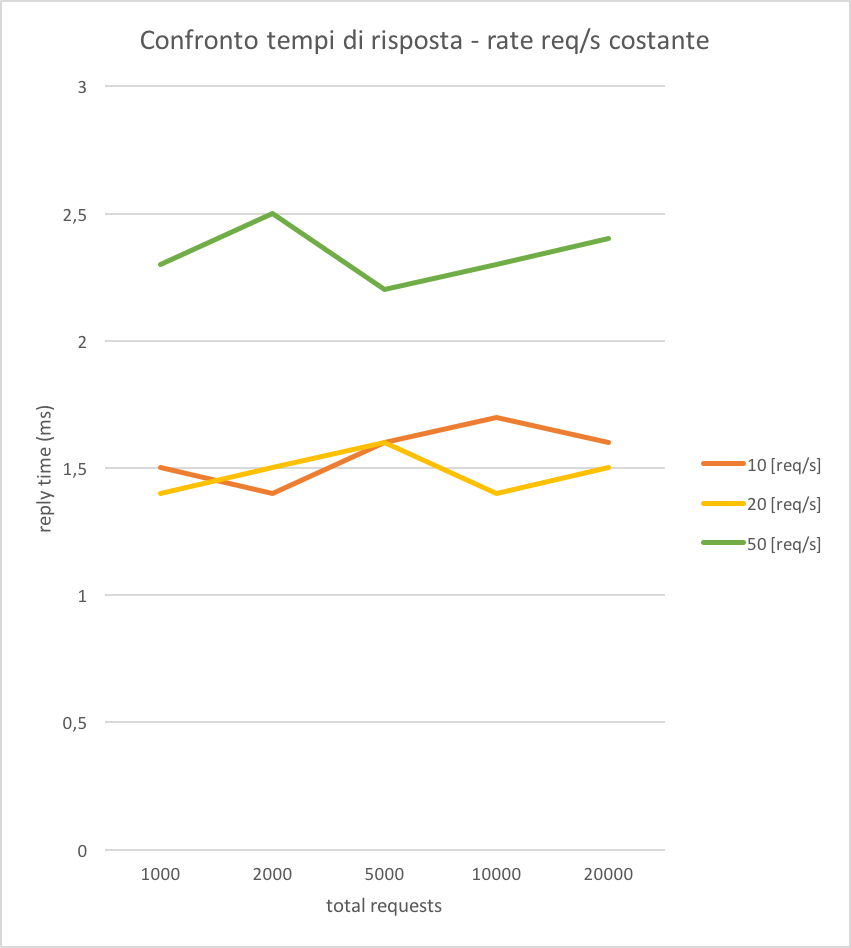
\includegraphics[width=\textwidth]{images/cfr_reply_time1}
\caption{Confronto fra i tempi di risposta con diversi rate all'aumentare delle richieste. Si osserva lo stabilizzarsi intorno ad un livello medio.\label{fig: cfr_reply_time1}}
\end{figure}\begin{figure}[H]
\centering
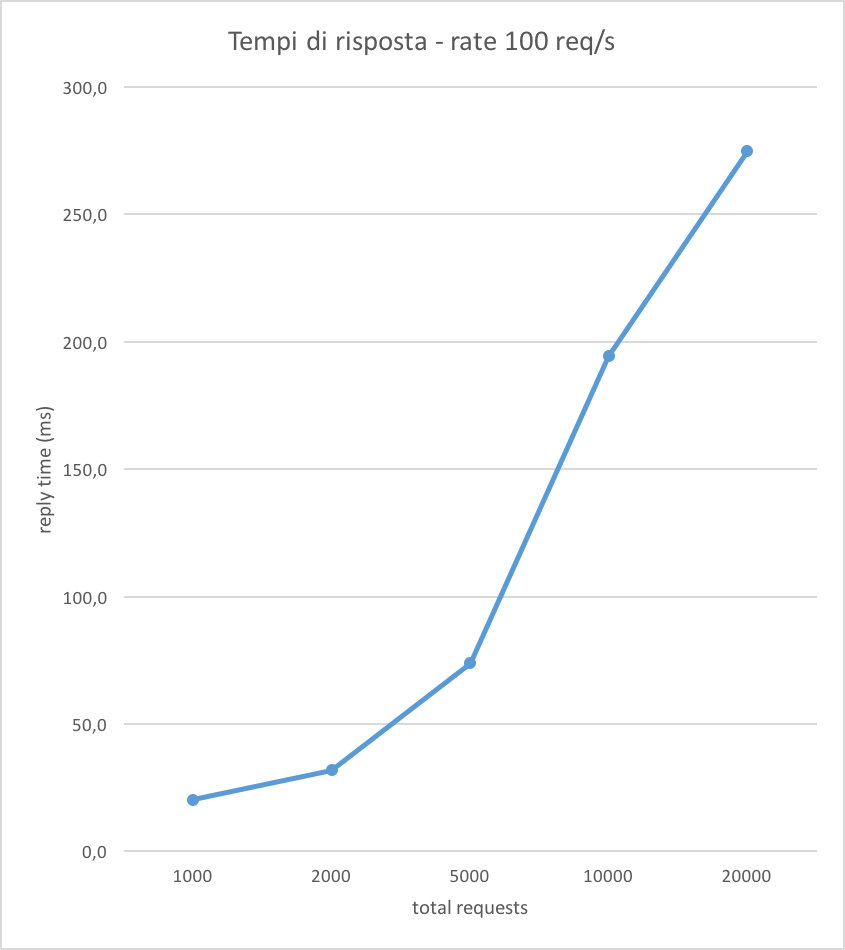
\includegraphics[width=\textwidth]{images/cfr_reply_time2}
\caption{Crescita dei tempi di risposta all'aumentare del numero di richiesta, si osserva come il lavoro dei worker non è sufficiente è compensare la frequenza delle richieste. \label{fig: cfr_reply_time2}}
\end{figure}
\subsection{Valutazione delle performance}
In questo caso abbiamo deciso di testare il programma in un possibile scenario applicativo vicino a quello di uno sviluppatore indipendente o di uno studente. Valutando le dimensioni tipiche di un \emph{Virtual Private Server} di fascia \emph{entry level}, abbiamo utilizzato una macchina virtuale con 512 MB di RAM con sistema operativo Ubuntu Server. Le condizioni del test includevano un numero di richieste fisso pari a 10000 richieste in arrivo, facendo variare la frequenza con cui queste giungevano. Si è deciso di prendere in considerazione sia il tempo di risposta che la frequenza con cui queste risposte giungevano al client che generava il carico di lavoro. \\\\ 
Quello che si è potuto constatare, relativamente alla \emph{figura \ref{fig: reply_times}}, è il crescere dei tempi di risposta linearmente, con un andamento paragonabile a quello osservato ma in questo caso riconducibile ad un carico di richieste al secondo, piuttosto che all'aumentare delle connessioni. Difatti si ha, mantenendo le connessioni costanti, il raggiungimento di un livello medio attorno al quale rimangono, a meno di oscillazioni, apprezzabili i tempi di risposta. Si può dedurre l'esistenza di un livello di saturazione che non può essere ne abbattuto, a causa della frequenza elevata, ne innalzato a causa della frequenza fissa con il quale i worker si liberano e vengono rioccupati da nuove connessioni. Tale frequenza di lavoro è dovuta sia alla presenza di una coda delle richieste che garantisce una certa inerzia, sia al raggiunto limite delle capacità della macchina di operare il context switching e nel ricreare i thread. \\\\
In \emph{figura \ref{fig: reply_freq}}, invece, è possibile osservare come, ad un livellarsi dei tempi di risposta, corrisponde, all'aumentare della frequenza di invio delle richieste, un aumento della frequenza di ricezione delle risposte. Il che ci porta a concludere che a pieno regime il web switch riesce ad adeguarsi alla velocità con cui sono in arrivo le richieste e soddisfare la domanda, seppure con un ritardo medio nei tempi di risposta.
\begin{figure}[H]
\centering
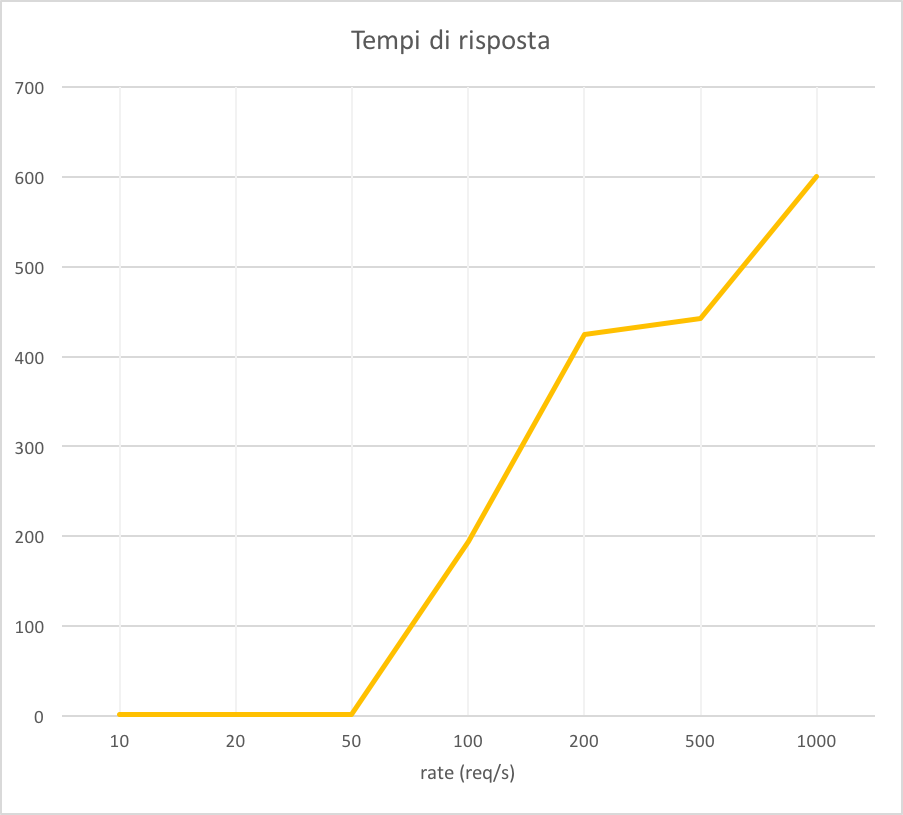
\includegraphics[width=\textwidth]{images/reply_times}
\caption{Analisi dei tempi di risposta all'aumentare del numero di richieste per secondo.\label{fig: reply_times}}
\end{figure}
\begin{figure}[H]
\centering
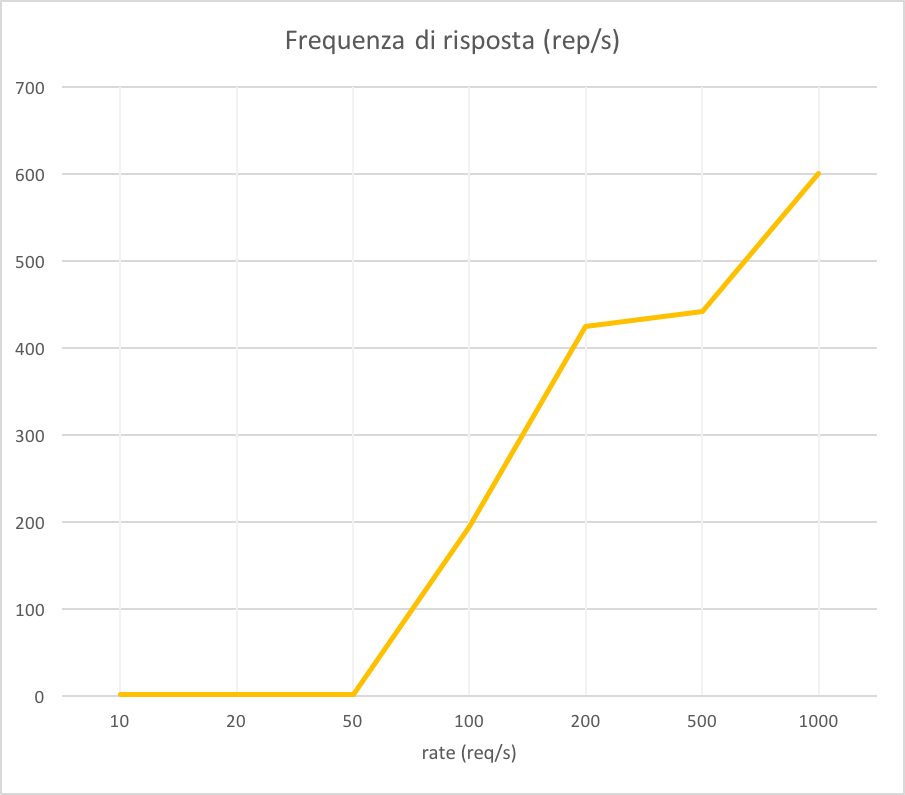
\includegraphics[width=\textwidth]{images/reply_freq}
\caption{Analisi della frequenza di risposta.\label{fig: reply_freq}}
\end{figure}
\subsection{Comparazione con Apache}
Con le caratteristiche della macchina di test già riportate nella sezione precedente, si è proceduto a verificare, una volta valutate le performance a regime, quale fosse l'overhead aggiunto dal nostro programma ad una delle macchine del cluster montante un web server Apache. \\
Possiamo verificare le statistiche di questo test alla \emph{figure \ref{fig: apachevsheimdall}}. Si osserva come, malgrado i tempi di risposta siano inferiori, tale differenza diventa poco apprezzabile nel momento in cui si ha una maggiore frequenza nelle risposte da parte del web server Apache. In conclusione si osserva come la durata del test è, in entrambi i casi, irrisoria e confrontabile. Per cui l'overhead aggiunto, per quanto non possa essere eccessivamente abbattuto, risulta essere accettabile per un'applicazione effettiva del web switch.
\begin{figure}[H]
\centering
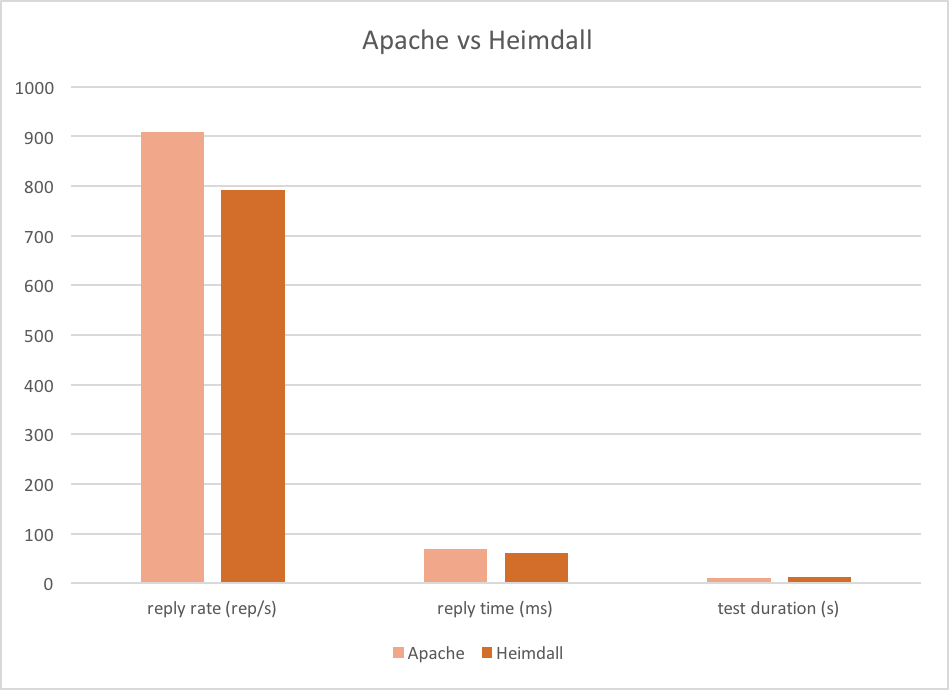
\includegraphics[width=\textwidth]{images/apachevsheimdall}
\caption{Confronto dei tempi di risposta di un web server Apache con il web switch Heimdall(10000 richieste per una frequenza di 100 req/s).\label{fig: apachevsheimdall}}
\end{figure}
\subsection{Limitazioni}
Durante i test che sono appena stati descritti, in particolare quelli con macchina virtuale, monitorando anche le risorse della macchina, si è potuto constatare che era presente un'\textbf{occupazione della RAM} crescente e, in alcuni casi, eccessiva, al punto da non permettere alla macchina di proseguire ulteriormente nelle operazioni. Tale occorrenza, per quanto rara e verificabile solamente nel caso di un carico veramente elevato, è dovuta alla non corretta liberazione della memoria nei processi che agiscono da worker: un'analisi più accurata ha portato alla luce la presenza di una grande quantità di memoria virtuale allocata e liberata correttamente ma, con una frequenza elevata di richieste in arrivo, non viene liberata memoria con la stessa velocità con cui viene occupata, portando ad una situazione pericolosa di saturazione. \\
Ben altra saturazione è stata evitata, invece, limitando il \textbf{numero di file descriptor} associabili ad una socket, imponendo alla macchina di rispettare un certo limite ed evitando, quindi, di portare il programma al blocco nel caso di termine delle risorse a disposizione del processo. \\\\
E' possibile apprezzare in \emph{figura \ref{fig: fd_memory}} l'occupazione di memoria e di file descriptor durante uno \emph{stress test} poco prima del raggiungimento del limite di memoria a disposizione. 
\begin{figure}[H]
\centering
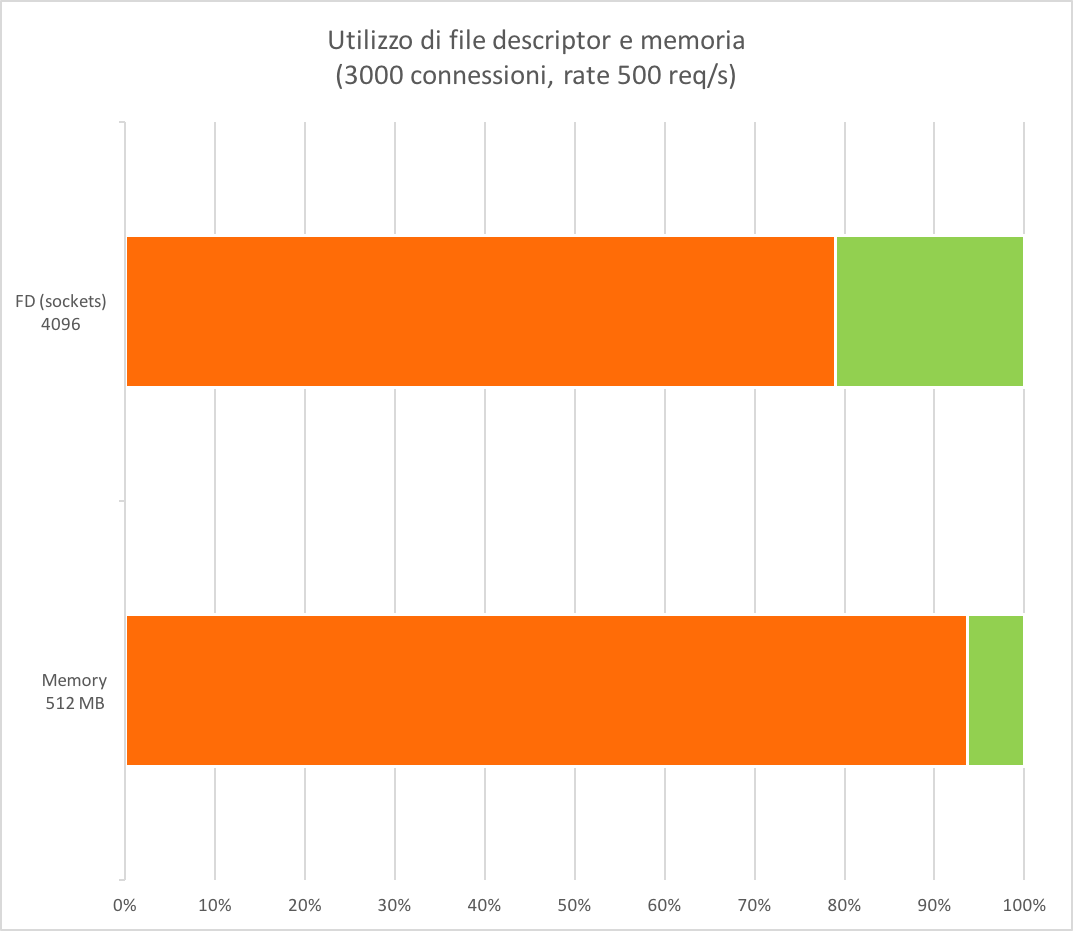
\includegraphics[width=\textwidth]{images/fd_memory}
\caption{Visualizzazione dell'occupazione di memoria e fd durante uno stress test.\label{fig: fd_memory}}
\end{figure}
\subsection{Conclusioni}
\newpage
\section{Future implementazioni}
\subsection{Analisi della richiesta}
Come abbiamo già visto nei paragrafi dedicati al \emph{parsing} delle richieste e delle risposte HTTP, è stato possibile, in fase progettuale, scegliere su quali \emph{header} basare il funzionamento elementare del web switch. Abbiamo visto anche come i file di configurazione garantiscono veramente molta flessibilità al sistemista in sede di installazione. \\
Non è difficile immaginare che, in una futura implementazione, l'applicazione non possa basarsi su file di configurazione più dettagliati e quindi possibilità di utilizzare tutti i parametri a disposizione per l'analisi di richiesta e risposta. Per cui si aprono scenari in cui si possono, ad esempio, configurare server di \emph{cache di immagini} in particolari posizioni del cluster, oppure utilizzare un algoritmo di schedulazione \emph{state-aware} che si basi anche sulla grandezza dei file richiesti e che quindi, a monte, eviti il carico di macchine sensibili.
\subsection{Webserver performante}


% --- References ---  
%
% bibtex is used to generate the bibliography. The babplain style
% will generate numeric references (e.g. [1]) appropriate for theoretical
% computer science. If you need alphanumeric references (e.g [Tur90]), use
%
% \bibliographystyle{babalpha-lf}
%
% instead.


\newpage
%\bibliographystyle{babplain-lf}
%\bibliography{references}
\renewcommand{\refname}{\normalfont\selectfont\normalsize\textbf{Annotazioni}} 
\begin{thebibliography}{9}
\bibitem{lamport94}
  Leslie Lamport,
  \emph{\LaTeX: a document preparation system},
  Addison Wesley, Massachusetts,
  2nd edition,
  1994.
  
\end{thebibliography}

% --- Appendices --- 
\newpage
\appendix
\newpage
\section{Manuale per l'uso}
\newpage
\section{Vagrant}

Durante lo sviluppo ci siamo imbattuti in alcune problematiche
legate alla portabilità del codice che stavamo scrivendo, errori di inclusione di file header, funzioni con comportamenti anomali, macro differenti e problemi nella compilazione. Questo perché lo sviluppo procedeva su macchine con sistemi operativi differenti, nello specifico Mac OSX e Debian. Da qui la necessità di avere un ambiente unificato per l'esecuzione del codice. La soluzione al problema era di facile intuizione, creare una macchina virtuale su VirtualBox e distribuirla su tutti i computer utilizzati per lo sviluppo, purtroppo però mettere in piedi questa soluzione può rivelarsi un'operazione tediosa, installazione del sistema operativo, configurazione dei programmi per lo sviluppo e condivisione di una VM che pesa diversi MB.\\\\
\textbf{Vagrant} è uno strumento per la creazione di ambienti di sviluppo completo. Fondamentalmente si tratta di un’applicativo scritto in Ruby che sfruttando le API messe a disposizione da VirtualBox è in grado di manipolare la gestione delle macchine virtuali al suo interno. Il tutto semplicemente compilando una "ricetta" chiamata Vagrantfile. Il \textbf{Vagrantfile} è un file all’interno del quale si inseriscono tutte le specifiche riguardo la VM che vogliamo preparare, impostando il sistema operativo, ulteriori programmi da installare, cartelle condivise, configurazioni di rete e quant'altro. Una volta preparato il vagrantfile questo può essere condiviso tra tutti gli sviluppatori, quindi senza dover condividere l'intera VM basterà solo questo file per poter avere tutte le macchine virtuali allo stesso stato. Ogni volta che uno sviluppatore avrà necessità di modificare il comportamento della VM basterà modificare il Vagrantfile e condividerlo con gli altri. Ultima caratteristica è che vagrant è pensato per lasciare allo sviluppatore la scelta dell'IDE che preferisce creando un ambiente completamente trasparente per lo sviluppo del software.\\\\
\emph{Vagrant makes the "works on my machine" excuse a relic of the past.}

\newpage
\section{Cluster virtuale}

\newpage
\section{Tool per i debug}
\subsection{GDB}
\subsection{Valgrind}

\newpage
% TODO check for download links
\section{Tool per i test}
In fase di sviluppo è necessario eseguire molteplici test prima di poter dare per \emph{certificato} il corretto funzionamento di un componente del programma. Nel nostro caso non è stata tanto la quantità dei test l'elemento caratterizzante, quanto la necessità di compiere questi test in un set molto variegato di casi. \\\\
Andiamo ora a vedere nel dettaglio quali sono stati i \emph{tool} che ci hanno permesso prima di verificare la corretta risposta del web switch all'arrivo di una richiesta secondo protocollo HTTP/1.1, quindi di aumentare il livello di complessità: dalla corretta ricezione di un file da un server remoto fino al funzionamento in condizioni di ideali utilizzo (via browser da parte di un client qualsiasi), passando per le condizioni di stress da carico nell'analisi delle performance.
\subsection{Telnet}
In questo caso ci si riferisce al programma da linea di comando che, implementando il protocollo di rete omonimo lato client, permette di instaurare una sessione di login verso un host remoto. Nel nostro caso ci ha permesso di eseguire il \emph{debugging} della risposta ad un regolare, semplificato, pacchetto HTTP. E' possibile utilizzare un client telnet da qualsiasi sistema operativo, inoltre è già presente nella maggior parte delle distribuzioni Linux.
\begin{lstlisting}
$ telnet localhost 8080
Trying 127.0.0.1...
Connected to localhost.
Escape character is '^]'.
GET / HTTP/1.1
Host: 127.0.0.1

\end{lstlisting}
\subsection{PostMan}
Questa è una applicazione presente nel \emph{Chrome Web Store} e che gira come plug-in del famoso browser Google Chrome. E' concepita come tool per testare le API, in particolare permette di specificare una richiesta HTTP con focus su quelli che sono i parametri ed i metodi specifici del protocollo. Nel nostro caso ha permesso di costruire un pacchetto base HTTP e verificare la corretta risposta del web switch al variare dei parametri. Potendo, inoltre, concentrarci su un singolo file da richiedere al server remoto, si è potuto sfruttare PostMan per analizzare i tempi di risposta, soprattutto in condizioni di file di grandi dimensioni.
\subsection{HttPerf} \label{ssec: httperf}
E' un tool per misurare le performance di un server web, svilupatto dai laboratori della HP. E' stato usato per generare diversi set di carico di lavoro da sottoporre al web switch per analizzarne le performance. Questo strumento è particolarmente versatile e permette di specificare tutta una serie di parametri come il \emph{numero di connessioni}, il \emph{numero di richiesto}, il \emph{rate} con cui effettuare tali connessioni, la \emph{risorsa} da richiedere, nonchè la possibilità di aprire un numero necessario di porte TCP per verificare la risposta di un certo carico di lavoro durante una sessione.
\begin{lstlisting}
$ httperf --server=localhost --uri=/index.html --port=8080
          --num-conns=3000 --num-calls=2 --rate=500

\end{lstlisting}
\subsection{Browser}
\begin{figure}[h]
\centering

\includegraphics[width=\textwidth]{images/screen_browser}
\caption{Schermata con la richiesta, soddisfatta con successo, del sito ospitato durante lo sviluppo su una delle macchine del cluster (browser utilizzato: Mozilla Firefox)}
\end{figure}
Questo è il tool principe per quanto riguarda il test "finale" del web switch: ci permette di verificare che l'esperienza utente nell'utilizzo di Heimdall nell'inoltrare le richieste ad un clsuter è confrontabile con una richiesta diretta ad una delle macchine del cluster stesso. Tuttavia in fase di sviluppo ci si è scontrati con le caratteristiche proprie di ciascun browser, per poterne valutare le performance. \\
Ci si è imbattuti innanzitutto nella funzionalità di \emph{pipelining} disabilitata di default su \textbf{Firefox} ma che è possibile abilitare, oppure l'apertura di diverse connessioni con il server entro le quali vengono effettuate molteplici richieste come \emph{Chrome} o \emph{Safari} o, generalmente, un qualsiasi browser moderno. \\\\
E' possibile osservare tali peculiarità, durante la richiesta verso un sito mediamente complesso, come quello utilizzato durante i test, dal listato sottostante, preso dai \emph{file di log durante una navigazione verso l'homepage con Chrome Web Browser}.
\begin{lstlisting}[basicstyle=\fontsize{4}{7}\selectfont\ttfamily]

Wed Feb 10 12:10:58 2016] - 192.168.1.3:8080 to: 192.168.1.5 - worker: 6882 - GET /font-awesome/css/font-awesome.min.css HTTP/1.1
[Wed Feb 10 12:10:58 2016] - 192.168.1.3:8080 to: 192.168.1.6 - worker: 6881 - GET /css/animate.min.css HTTP/1.1
[Wed Feb 10 12:10:58 2016] - 192.168.1.3:8080 to: 192.168.1.4 - worker: 6883 - GET /js/bootstrap.min.js HTTP/1.1
[Wed Feb 10 12:10:58 2016] - 192.168.1.3:8080 to: 192.168.1.5 - worker: 6879 - GET /js/jquery.easing.min.js HTTP/1.1
[Wed Feb 10 12:10:58 2016] - 192.168.1.3:8080 to: 192.168.1.5 - worker: 6882 - GET /js/jquery.fittext.js HTTP/1.1
[Wed Feb 10 12:10:58 2016] - 192.168.1.3:8080 to: 192.168.1.4 - worker: 6880 - GET /js/wow.min.js HTTP/1.1
[Wed Feb 10 12:10:58 2016] - 192.168.1.3:8080 to: 192.168.1.6 - worker: 6881 - GET /js/creative.js HTTP/1.1
[Wed Feb 10 12:10:58 2016] - 192.168.1.3:8080 to: 192.168.1.6 - worker: 6878 - GET /img/portfolio/2.jpg HTTP/1.1
[Wed Feb 10 12:10:58 2016] - 192.168.1.3:8080 to: 192.168.1.4 - worker: 6883 - GET /img/portfolio/4.jpg HTTP/1.1
[Wed Feb 10 12:10:58 2016] - 192.168.1.3:8080 to: 192.168.1.5 - worker: 6879 - GET /img/portfolio/5.jpg HTTP/1.1
[Wed Feb 10 12:10:58 2016] - 192.168.1.3:8080 to: 192.168.1.4 - worker: 6880 - GET /img/portfolio/6.jpg HTTP/1.1
[Wed Feb 10 12:10:58 2016] - 192.168.1.3:8080 to: 192.168.1.4 - worker: 6883 - GET /img/header.jpg HTTP/1.1
[Wed Feb 10 12:10:58 2016] - 192.168.1.3:8080 to: 192.168.1.4 - worker: 6883 - GET /font-awesome/fonts/fontawesome-webfont.woff?v=4.3.0 HTTP/1.1
[Wed Feb 10 12:10:58 2016] - 192.168.1.3:8080 to: 192.168.1.4 - worker: 6877 - GET /favicon.ico HTTP/1.1

\end{lstlisting}

\newpage
\begin{figure}[c]
\centering
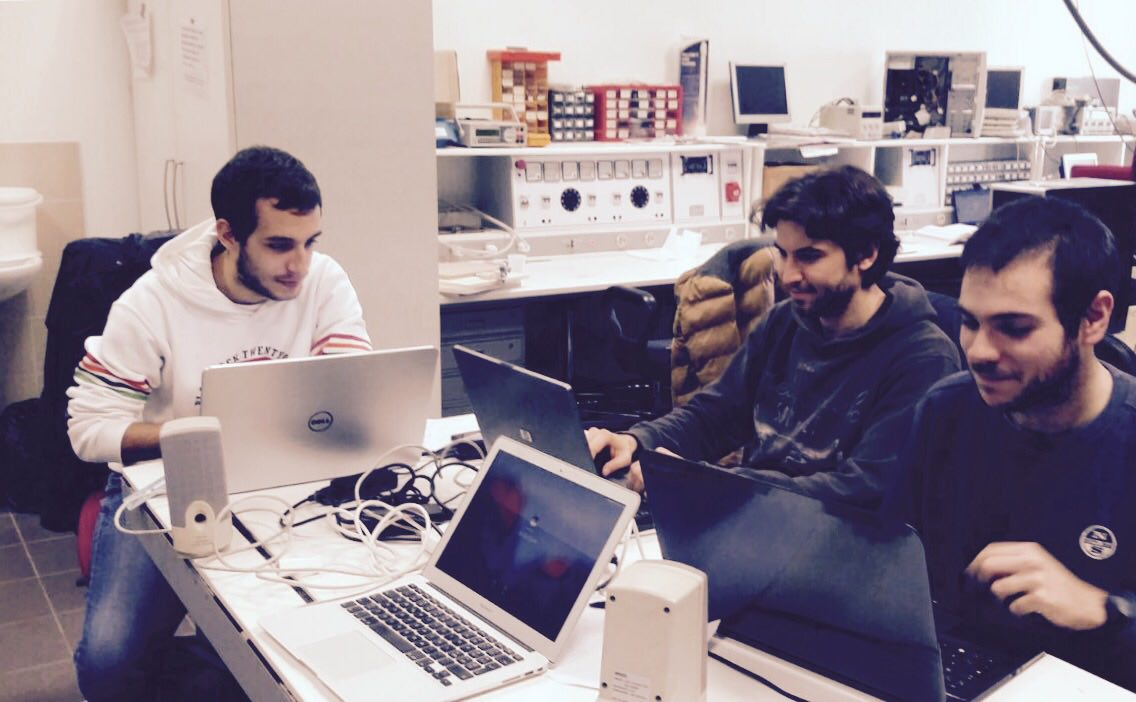
\includegraphics[width=\textwidth]{images/team}
\caption{Il team di sviluppo del Progetto Heimdall durante i test del web switch a pieno regime (\emph{febbraio 2016, Laboratori di Tor Vergata})}
\end{figure}


\end{document}